\section{Conditional Probability}
Let $A$ be an event. Recall that $\PR(A)$ is the probability that $A$ occurs. Now, suppose that we're given some additional information. Then, this information may not completely determine whether $A$ has occurred, but it might give us some valuable partial information. 

\begin{mdframed}[]
    (Example.) Suppose that a magician rolls a fair die. Let $A$ be the event that we roll a 6. Then, we know that 
    \[\PR(A) = \frac{1}{6}.\]
    Now, let's suppose that the magician tells you that the result is an even number (either 2, 4, or 6), but does not yet reveal the full result of the roll to you. How does the probability of $A$ change? It's certainly not $\frac{1}{6}$ since we know that it has to be an even number. Intuitively, the answer is $\frac{1}{3}$; this is particularly because the die originally was uniform, so there is no reason why -- when the magician got an even number -- the even numbers have a heavier weight. 
\end{mdframed}

\subsection{What is Conditional Probaiblity?}
Conditional probability is the study of probability under the presence of partial information. 
\begin{definition}{Conditional Probability}{}
    Let $A$ and $B$ be two events such that 
    \begin{itemize}
        \item $A$ is  the event of interest.
        \item $B$ is the event that encodes the partial information that we have. 
    \end{itemize}
    Suppose that $\PR(B) > 0$. Then, the \textbf{conditional probability} of $A$, given that $B$ has occurred, is denoted by $\PR(A | B)$.  
\end{definition}
\textbf{Remarks:} 
\begin{itemize}
    \item We require $\PR(B) > 0$; if $\PR(B) = 0$, then this would imply that $B$ would never occur anyways. 
    \item All of the given information is on the \emph{right} of the bar. 
\end{itemize}
In our example above, $A$ would be the event of interest and $B$ is the event coming from the magician telling us that the roll was an even number. 

\subsection{Finding Conditional Probability}
How do we find $\PR(A | B)$? 
\begin{mdframed}[]
    (Example, Continued.) In the previous example, it's clear that the probability of rolling a 6 should change from $\frac{1}{6}$ to $\frac{1}{3}$ once we found out that the roll is an even number. Additionally, the roll is uniformly random -- now, we know that there is one of \emph{three} possible numbers, so it should still remain uniformly random, but just on the sample space $\{2, 4, 6\}$ instead of the original sample space $\{1, 2, 3, 4, 5, 6\}$. 

    \bigskip 

    So, if $A$ is the event that we rolled a 6, and $B$ is the even that we rolled an even number, notice that: 
    \begin{itemize}
        \item $\PR(A) = \frac{1}{6}$: This is the probability that we roll a 6.
        \item $\PR(B) = \frac{1}{2}$: This is the probability that we will any even number.
        \item $\PR(A \cap B) = \frac{1}{6}$: This is the probability that both events occur. Notice that $A$ is a subset of $B$; therefore, $A \cap B = A$. 
    \end{itemize}
    Intuitively, we expect $\PR(A | B) = \frac{1}{3}$, and indeed we note that 
    \[\frac{\PR(A \cap B)}{\PR(B)} = \frac{1 / 6}{1 / 2} = \frac{1}{3}.\]
\end{mdframed}
In general, it is true that 
\[\boxed{\PR(A | B) = \frac{\PR(A \cap B)}{\PR(B)}}.\]
Why is this true? 
\begin{mdframed}[]
    (Informal Discussion.) Suppose that the sample space is $\Omega$ and we have two events $A, B \subset \Omega$. Then, consider the following Venn Diagram, where $\PR(A)$ is represented by $\frac{\text{area}(A)}{\text{area}(\Omega)}$ and $\PR(B)$ is represented by $\frac{\text{area}(B)}{\text{area}(\Omega)}$. 
    \begin{center}
        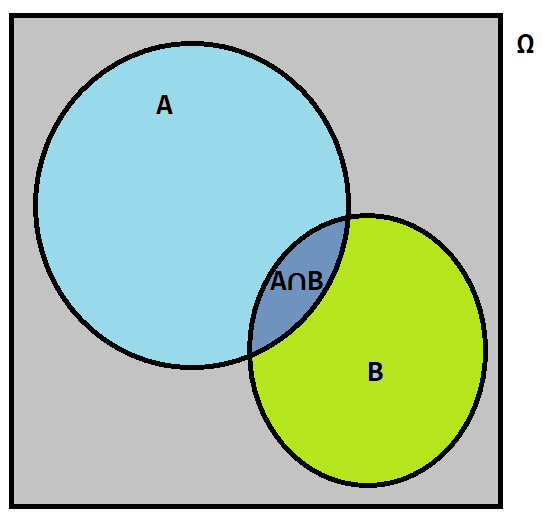
\includegraphics[scale=0.7]{assets/venn1.png}
    \end{center}
    Now, the idea is that when we randomly throw a dart at the ``dartboard'' $\Omega$, it will ``land in'' $A$ with probability $\PR(A)$ and similarly for $B$. 
    
    \bigskip 
    
    Now, suppose that we are told that the dart landed somewhere in $B$, but we don't know anything else beyond that. Then, since the dart was thrown randomly, it should be in some random position in $B$ (i.e. nowhere in $B$ should be more likely than anywhere else). Now, what is the probability that it landed in $A$, \emph{given} that it landed somewhere in $B$?
    \begin{center}
        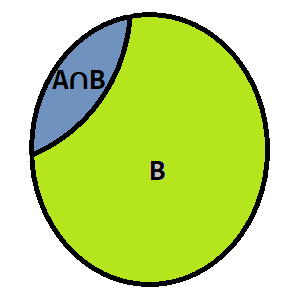
\includegraphics[scale=0.7]{assets/venn2.png}
    \end{center}
    The answer is to find out what is the probability that the dart landed in the intersection, that is, in the $A \cap B$ region. In this case, we can consider their \emph{ratios} -- in this case, we consider the area of $A \cap B$ against the area of $B$. Then, in effect, $B$ becomes the new sample space (i.e. the ``dartboard''), since we now know that the outcome of the experiment is in $B$. Therefore, we have 
    \[\PR(A | B) = \frac{\PR(A \cap B)}{\PR(B)}.\]
\end{mdframed}
With this in mind, we can now give a formal definition.
\begin{definition}{Conditional Probability}{}
    Let $A$ and $B$ be two events. Suppose that $\PR(B) > 0$. Then, the \textbf{conditional probability} of $A$, given that $B$ has occurred, is $\PR(A | B) = \frac{\PR(A \cap B)}{\PR(B)}$.  
\end{definition}
Recall that $\PR(\omega)$ is a probability distribution on the sample space $\Omega$ \emph{if} we have 
\begin{itemize}
    \item $\PR(\omega) \geq 0$ for all $\omega \in \Omega$, and 
    \item $\sum_{\omega \in \Omega} \PR(\omega) = 1$. 
\end{itemize}
Note that the function $\PR(\omega | B)$ is \emph{also} a probability distribution, but now the \emph{sample space} is $B$. In particular:
\begin{enumerate}
    \item $\PR(\omega | B) = \frac{\PR(\omega \cap B)}{\PR(B)} = \frac{\PR(\omega)}{\PR(B)} \geq 0$ for all $\omega \in B$. Note that this is true since $\PR(B) > 0$ and $\PR(\omega) \geq 0$ for all $\omega \in \Omega$. 
    \item $\sum_{\omega \in B} \PR(\omega | B) = \frac{1}{\PR(B)} \sum_{\omega \in B} \PR(\omega) = \frac{1}{\PR(B)} \PR(B) = 1$. 
\end{enumerate}
Note that, by multiplying both sides of the conditional probability formula $P(A | B)$ by $P(B)$, we get the following formula:
\begin{theorem}{Probability Chain Rule}{}
    \[\PR(A \cap B) = \PR(B) \PR(A | B).\]
\end{theorem}
\textbf{Remarks:}
\begin{itemize}
    \item The conditional probability formula only holds when $\PR(B) > 0$. 
    \item The probability chain rule $\PR(A \cap B) = \PR(B) \PR(A | B)$ holds even when $\PR(B) = 0$. 
\end{itemize}

\begin{mdframed}[nobreak=true]
    (Example.) On sunny days, Vito goes for a walk with probability $\frac{4}{5}$. On rainy days, Vito goes for a walk with probability $\frac{1}{10}$. Suppose that, in San Diego, it rains on any given day with probability $3\%$. Find the probability that Vito goes for a walk today. 

    \begin{mdframed}[]
        We let $W$ be the event that Vito goes for a walk today; we want to find $\PR(W)$. Let $S$ be the event that it is sunny today.

        \bigskip 

        We know that it rains with a $3\%$ chance, so the change of it being sunny is $97\%$, or $\frac{97}{100}$. Thus, $\PR(S) = \frac{97}{100}$. We also know that the probability that Vito goes for a walk, \emph{given} that it is sunny\footnote{Note that we were not told that the probability of him going for a walk \emph{and} it being sunny is $\frac{4}{5}$; all we're told is that \emph{if} it is a sunny day, then he'll go for a walk with probability $\frac{4}{5}$.}, is $\PR(W | S) = \frac{4}{5}$. Likewise, the probability that Vito goes for a walk, given that it is rainy (not a sunny day), is $\PR(W | S^C) = \frac{1}{10}$. 

        \bigskip 

        Recall that, by the Law of Total Probability, we have 
        \[\PR(W) = \PR(W \cap S) + \PR(W \cap S^C) \implies \PR(W \cap S) = \PR(W) - \PR(W \cap S^C).\]
        Additionally, we know that 
        \[\PR(W \cap S^C) = \PR(S^C) \PR(W | S^C) = \frac{3}{100} \frac{1}{10} = \frac{3}{1000}.\]
        Therefore, applying this formula to the probability chain rule and solving, we get the following work: 
        \begin{equation*}
            \begin{aligned}
                \PR(W \cap S) &= \PR(S) \PR(W | S) && \text{Probability Chain Rule}\\ 
                    &\implies \PR(W) - \PR(W \cap S^C) = \PR(S) \PR(W | S) && \text{Applying Law of Total Probability} \\ 
                    &\implies \PR(W) = \PR(S) \PR(W | S) + \PR(W \cap S^C) && \text{Add } \PR(W \cap S^C) \text{ to Both Sides}\\ 
                    &\implies \PR(W) = \frac{97}{100} \frac{4}{5} + \frac{3}{1000} && \text{Substitute Values} \\ 
                    &\implies \PR(W) = \frac{779}{1000} && \text{Simplify}
            \end{aligned}
        \end{equation*}
    \end{mdframed}
\end{mdframed}

\subsection{Law of Total Probability, Conditional Version}
Recall that, if $A \subset \Omega$ is an event, and if $B_1, \dots, B_n$ are partitions of $\Omega$, then, the Law of Total Probability is given by  
\[\PR(A) = \sum_{i = 1}^{n} \PR(A \cap B_i).\]
Using the probability chain rule, we have
\[\PR(A) = \sum_{i = 1}^{n} \PR(B_i) \PR(A | B_i).\]
This is the conditional version of the Law of Total Probability.
\begin{theorem}{Law of Total Probability, Conditional Version}{}
    Suppose that $A \subset \Omega$ is an event and that the events $B_1, \dots, B_n$ partition that sample space $\Omega$. Then, we have that 
    \[\PR(A) = \sum_{i = 1}^{n} \PR(B_i) \PR(A | B_i).\]
\end{theorem}

\subsection{Independent Events}
Now that we have defined conditional probability, we can formally define what it means for events to be independent. 
\begin{definition}{Independent Events}{}
    Two events $A, B$ are \textbf{independent} if either 
    \begin{enumerate}
        \item $\PR(A) = 0$, 
        \item $\PR(B) = 0$, or 
        \item $\PR(A | B) = \PR(A)$ and $\PR(B | A) = \PR(B)$, in the case that both $\PR(A) > 0$ and $\PR(B) > 0$.
    \end{enumerate}
\end{definition}
\textbf{Remark:} With regards to (3), the occurrence of $B$ does not affect the occurrence of $A$, and vice versa. 

\bigskip 

Now, by the probability chain rule, if two events $A$ and $B$ are independent, then 
\[\PR(A \cap B) = \PR(A) \PR(B).\]
Indeed, $\PR(A \cap B) = \PR(A | B) \PR(B) = \PR(A) \PR(B)$. This introduces the next theorem: 
\begin{theorem}{}{}
    If $A$ and $B$ are independent, then 
    \[\PR(A \cap B) = \PR(A) \PR(B).\]
\end{theorem}

Now, independence is more complicated when more than two events are involved. In particular:
\begin{definition}{}{}
    Events $A_1, \dots, A_n$ are \textbf{mutually independent} if, for any $A_{i_1}, \dots, A_{i_k}$, we have that 
    \[\PR\left(\bigcap_{i = 1}^{k} A_{i_k} \right) = \prod_{i = 1}^{k} \PR(A_{i_k}).\]
\end{definition}
In particular, we have
\[\PR\left(\bigcap_{i = 1}^{n} A_{i} \right) = \prod_{i = 1}^{n} \PR(A_{i}).\]
A weaker version of independence is as follows: 
\begin{definition}{}{}
    Events $A_1, \dots, A_n$ are \textbf{pairwise independent} if each pair $A_i$, $A_j$ (with $i \neq j$) are independent.
\end{definition}
Note that if $n > 2$, then mutually and pairwise independence are \textbf{not} equivalent.

\bigskip 

So, in essense, the difference can be highlighted like so: 
\begin{itemize}
    \item Mutual independence: every event is independent of any intersection of the other events. 
    \item Pairwise independence: any two events are independent. 
\end{itemize}

\subsection{Joint Probability Distributions}
We now talk about joint probability distributions. 

\subsubsection{Joint PMFs}
Suppose that $X_1, \dots, X_n$ are discrete random variables with PMFs 
\[p_{X_i} = \PR(X_i = x).\]
Then, the joint PMF of the RV $\mathbf{X} = (X_1, \dots, X_n)$ is the function 
\[p_{\mathbf{X}}(x_1, \dots, x_n) = \PR(X_1 = x_1, \dots, X_n = x_n)\]
for all $x_1, \dots, x_n$. Here, we can think of this as a function from a sample space to $\R^n$ (higher dimensions).

\bigskip 

Often, it can be quite difficult to find the joint PMFs. However, in the special case that $X_1, \dots, X_n$ are \textbf{independent}, it is just the product of the individual PMFs; that is, 
\[p_{\mathbf{X}}(x_1, \dots, x_n) = \prod_{i = 1}^{n} p_{X_i}(x_i).\]
We say that $X_1, \dots, X_n$ are \textbf{independent and identically distributed}\footnote{This is known as \textbf{independent trial process} in the textbook.} (IID for short) if they are mutually independent, and all have the same distribution. 

\begin{mdframed}[]
    (Example.) Consider a sequence $X_1, \dots, X_n$ of $n$ Bernoulli($p$) trials. In this case, each trial has the simple distribution 
    \[\PR(X_i = 1) = p\]
    and 
    \[\PR(X_i = 0) = 1 - p.\]
\end{mdframed}

\subsubsection{Joint PDFs}
In general, though, in such a process, $X_i$ can have any given distribution. In any case, if $X_1, \dots, X_n$ are IIDs, then their joint PDF takes the simple form known as a \textbf{product distribution}. In particular, since the $X_i$'s are IIDs, they have the same PDFs $p(x) = \PR(X_i) = x$ no matter what $i$ is. Hence, the joint PDF is just 
\[\PR(X_1 = x_1, \dots, X_n = x_n) = \prod_{i = 1}^{n} p(x_i).\]

\begin{mdframed}[]
    (Example.) For example, in a sequence of Bernoulli($p$) trials, 
    \[\PR(X_1 = x_1, \dots, X_n = x_n) = p^k (1 - p)^{n - k},\]
    if exactly $k$ of the $x_i = 1$ and the other $n - k$ of the $x_i = 0$. 
\end{mdframed}


\begin{mdframed}[]
    (Example Problem.) Let $X, Y$ be independent Bernoulli($1/2$) random variables. Let $Z$ be a random variable that takes the value 1 if $X + Y = 1$, and 0 otherwise. Show that $X, Y, Z$ are pairwise, but not mutually, independent.

    \begin{mdframed}[]
        Trivially, we know that $\PR(X = 1) = \PR(X = 0) = \frac{1}{2}$ and $\PR(Y = 1) = \PR(Y = 0) = \frac{1}{2}$, since these are just Bernoulli($1/2$) random variables. We know that $X$ and $Y$ are both independent, so the values that they take do not affect each other. Using a table, we can fill out some possible values of $X$, $Y$, and $Z$. 
        \begin{center}
            \begin{tabular}{c|c|c|c}
                $\mathbf{X}$ & $\mathbf{Y}$ & $\mathbf{X + Y}$ & $\mathbf{Z}$ \\ 
                \hline 
                0 & 0 & 0 & 0 \\ 
                0 & 1 & 1 & 1 \\ 
                1 & 0 & 1 & 1 \\ 
                1 & 1 & 2 & 0 
            \end{tabular}
        \end{center}
        Since $X$ and $Y$ are independent, it follows that 
        \[p_{X, Y}(x, y) = p_{X}(x) p_{Y}(y) = \frac{1}{2} \frac{1}{2} = \frac{1}{4}.\]
        Recall that random variables $X_1, \dots, X_n$ are independent if
        \[p_{X_1, \dots, X_n}(x_1, \dots, x_n) = p_{X_1}(x_1) \dots p_{X_n}(x_n).\]
        From the table above, we know that 
        \[\PR(Z = 1) = \PR(Z = 0) = \frac{1}{2}.\]
        Now, recall that 
        \[p_{X, Z}(x, z) = \PR(X = x, Z = z).\]
        For any selection of $(x, z) \in \{(0, 0), (0, 1), (1, 0), (1, 1)\}$, we have 
        \[p_{X, Z}(x, z) = \frac{1}{4}.\]
        Likewise, we have that 
        \[p_{X}(x) = \frac{1}{2}\]
        and 
        \[p_{Z}(z) = \frac{1}{2}.\]
        Therefore, 
        \[p_{X, Z}(x, z) = \frac{1}{4} = \left(\frac{1}{2}\right)^2.\]
        However, note that we simply have $p_{X, Z}(x, z) = p_{X}(x) p_{Z}(z)$, so it follows that $X$ and $Z$ are pairwise independent. The same argument can be made for $Y$ and $Z$. Therefore, $X, Y, Z$ are pairwise independent. 
    
        \bigskip 
    
        Now, note that 
        \[p_{X, Y, Z}(0, 1, 1) = \frac{1}{4}.\]
        But, 
        \[p_{X}(0)p_{Y}(1)p_{Z}(1) = \frac{1}{2}\frac{1}{2}\frac{1}{2} = \frac{1}{8}.\]
        Since $p_{X, Y, Z}(0, 1, 1) \neq p_{X}(0)p_{Y}(1)p_{Z}(1)$, clearly $X, Y, Z$ are not mutually independent. 
    \end{mdframed}
\end{mdframed}



\subsection{Bayes' Formula}
Bayes' Formula is a powerful -- and very famous -- application of the conditional probability formula. Often, it can be difficult to calculate a conditional probability $\PR(A | B)$ of interest. However, the other way around, $\PR(B | A)$, could be easier to find. Bayes' Formula gives us a way of finding $\PR(A | B)$, provided that we know $\PR(A)$, $\PR(B)$, and $\PR(B | A)$. Recall that the conditional probability formula is given by 
\[\PR(A | B) = \frac{\PR(A \cap B)}{\PR(B)}.\]
We also know that 
\[\PR(B | A) = \frac{\PR(A \cap B)}{\PR(A)}.\]
So, solving for $\PR(A \cap B)$, we have 
\[\PR(A \cap B) = \PR(A | B) \PR(B) \qquad \PR(A \cap B) = \PR(B | A) \PR(A).\]
Then, setting these terms equal to each other, we have 
\[\PR(A | B) \PR(B) = \PR(B | A) \PR(A).\]
Thus, we get 
\[\boxed{\PR(A | B) = \frac{\PR(A) \PR(B | A)}{\PR(B)}}.\]
It is often useful to apply the conditional Law of Total Probability in the denominator; that is,
\[\PR(B) = \PR(A) \PR(B | A) + \PR(A^C) \PR(B | A^C).\]
So, sometimes, Bayes' Rule is stated like so:
\[\boxed{\PR(A | B) = \frac{\PR(A) \PR(B | A)}{\PR(A) \PR(B | A) + \PR(A^C) \PR(B | A^C)}}.\]
Now, there is a general version of Bayes' Rule; suppose that $B \subset \Omega$ is an event and $A_1, \dots, A_n$ partitions the sample space $\Omega$. Then, for each $1 \leq j \leq n$, we have 
\[\boxed{\PR(A_j | B) = \frac{\PR(A_j) \PR(B | A_j)}{\sum_{i = 1}^{n} \PR(A_i) \PR(B | A_i)}}.\]
Here\footnote{In this course, we aren't expected to memorize these.}, 
\begin{itemize}
    \item The $\PR(A_j)$ are called \textbf{prior probabilities}.
    \item The $\PR(A_j | B)$ are called \textbf{posterior probabilities}.
    \item The events $A_j$ are called \textbf{hypotheses}.
    \item The event $B$ is called the \textbf{evidence}.
\end{itemize}
Often, we want to see which hypothesis is more likely given the evidence.

\begin{mdframed}[]
    (Example.) Suppose that a doctor gives a patient a test for cancer. Before the test, all we know is that, on average, 1 in every 1000 women develop this cancer. According to the manufacturer, this test is $99\%$ accurate at detecting the cancer, when it is there. However, there is a $5\%$ chance it will show positive when the cancer is not there (i.e. there is a $1\%$ chance of a false negative, and a $5\%$ chance of a false positive). To make things more clear:
    \begin{itemize}
        \item If she has the cancer, there's a $1\%$ chance the test will incorrectly say negative, and a $99\%$ chance the test will correctly say positive. 
        \item If she does not have the cancer, there's a $5\%$ chance the test will incorrectly say positive.
    \end{itemize}
    Now, suppose that the patient tests positive. \emph{With what probability does she actually have the cancer?}

    \begin{mdframed}[]
        Let $C$ be the event that she has this cancer. Let $P$ be the event that this test is positive. We want to find $\PR(C | P)$. We know that 
        \[\PR(C) = 0.001 \qquad \PR(P | C) = 0.99 \qquad \PR(P | C^C) = 0.05.\]
        By Bayes' Rule, we have 
        \[\PR(C | P) = \frac{\PR(C) \PR(P | C)}{\PR(C) \PR(P | C) + \PR(C^C) \PR(P | C^C)} = \frac{0.001(0.99)}{0.001(0.99) + 0.999(0.05)} \approx 1.94\%.\]
    \end{mdframed}
\end{mdframed}
\textbf{Remark:} Given that the test is supposed to be $99\%$ accurate and that the patient tested positive, one would think that the patient has the cancer; so, a near $2\%$ probability that the patient has cancer is quite surprising. However, there are a few reasons why this may be the case.
\begin{enumerate}
    \item Even though the test is fairly accurate when you do have the cancer, when you don't have the cancer there is a decent chance ($5\%$) that it will be incorrect.
    \item This cancer is \emph{extremely} rare; it's so rare that there is a much better chance that this test will incorrectly read positive than if you actually have cancer. 
\end{enumerate}
Now, without any additional information (i.e. without the test), we could only assume that the patient had this cancer with probability $0.1\%$. After testing positive, this probability increases by quite a bit, but it is still only $1.94\%$. This example demonstrates that it is very difficult to design an accurate test for a rare disease; in this example, the probability of a false positive is much more likely than the patient actually having cancer.

\begin{mdframed}[]
    (Example Problem.) An airplane is missing. Based on its flight plan, it has been determined that the airplane is equally likely to be in any one of three locations (each with probability $1/3$). Some locations are easier to search than others for various geological reasons. If the airplane is in location $1,2,3$ then the team will find it while searching there with probability $1/2$, $1/3$, $1/4$, respectively. Suppose that location 1 is searched first, and the airplane is not found there. Show that, given this, with conditional probability $2/5$ the airplane is in location 2.

    \begin{mdframed}[]
        We will use Bayes' Formula,
        \[\PR(A | B) = \frac{\PR(B | A) \PR(A)}{\PR(B)},\]
        where $A$ is the event that the plane is in location 2 and $B$ is the event that the airplane was not found in location 1. We note that 
        \[\PR(\text{Plane in Loc. 1}) = \boxed{\PR(\text{Plane in Loc. 2}) = \PR(A)} = \PR(\text{Plane in Loc. 3}) = \frac{1}{3}.\]
        Let $L_i$ be the event that the plane is in location $i$. By the conditional law of total probability, we know that 
        \[\PR(B) = \PR(L_1) \PR(B|L_1) + \PR(L_2) \PR(B|L_2) + \PR(L_3) \PR(B|L_3).\]
        We now consider each case individually:
        \begin{itemize}
            \item Suppose the plane was in location 1, but the search occurred (and failed) in location 1. Since there was a $\frac{1}{2}$ chance that the plane could be found in location 1, then there is a $1 - \frac{1}{2} = \frac{1}{2}$ chance that the plane will not be found in location 1. So:
            \[\PR(L_1) \PR(B|L_1) = \frac{1}{3} \left(1 - \frac{1}{2}\right) = \frac{1}{6}.\]

            \item Suppose the plane was in location 2, but the search occurred in location 1. Note that if the plane was in location 2, then trivially there is a 100\% chance the plane will not be found in location 1, so it follows that $\PR(B|L_2) = \PR(B|A) = 1.$ Then:
            \[\PR(L_2) \PR(B|L_2) = \frac{1}{3} \cdot 1 = \frac{1}{3}.\]
            
            \item Suppose the plane was in location 3, but the search occurred in location 1. The same reason from the previous part can be applied to this part as well. Then:
            \[\PR(L_3) \PR(B|L_3) = \frac{1}{3} \cdot 1 = \frac{1}{3}.\]
        \end{itemize}
        Thus, $\PR(B) = \frac{5}{6}$. So, we have 
        \begin{equation*}
            \begin{aligned}
                \PR(A|B) &= \frac{\PR(B | A) \PR(A)}{\PR(B)} \\ 
                    &= \frac{1 \cdot 1/3}{5/6} \\ 
                    &= \frac{1}{3} \cdot \frac{6}{5} \\ 
                    &= \boxed{\frac{2}{5}}.
            \end{aligned}
        \end{equation*}
        Thus, we got the desired answer.
    \end{mdframed}
\end{mdframed}



\subsection{Conditional Probability: Continuous Case}
Conditional probability is slightly different in the ``world'' of continuous random variables. Most of the same definitions carry over from the discrete case, but since we're dealing with \emph{PDFs}\footnote{Remember, PDFs are not probabilities; they are densities. They allow us to get a probability by integrating, but they're not probabilities.} $f(x)$ instead of PMFs $p(x) = \PR(X = x)$ (which are probabilities, unlike PDFs).

\bigskip 

Recall that if $\PR(\omega)$ is a discrete probability distribution and $\PR(B) > 0$, then the distribution $\PR(\omega | B) = \frac{\PR(\omega)}{\PR(B)}$ is a probability distribution on $B$.
\begin{definition}{}{}
    Let $X$ be a continuous random variable with PDF $f$. Suppose that $B$ is an event with $\PR(B) > 0$. Then, the conditional PDF of $X$, given $B$, is 
    \[f(x | B) = \begin{cases}
        \frac{f(x)}{\PR(B)} & x \in B \\ 
        0 & x \notin B
    \end{cases}.\]
\end{definition}
We note that $f(x) \geq 0$ and 
\[\int_{-\infty}^{\infty} f(x | B) dx = \frac{1}{\PR(B)} \int_{B} f(x) dx = \frac{1}{\PR(B)} \PR(B) = 1.\]
Note that the integration over a region gives us the probability of being in that region, i.e. integrating $f(x)$ over the region $B$ gives us just $\PR(B)$. Therefore, $f(x | B)$ is indeed a probability density on $B$. 

\begin{mdframed}[]
    (Example.) Recall the spinner example. The location of the spinner, when it eventually comes to rest, is uniform on the unit circle; thus, 
    \[f(x) = 1 \text{ for } x \in [0, 1).\]
    Suppose that the spinner comes to rest in the upper-half of the circle, i.e. in $[0, 1/2]$. What is the (conditional) probability with which it lands in the region $[1/6, 2/3]$?

    \begin{mdframed}[]
        The probability of $B$ occurring (the event that the spinner lands in the upper-half of the circle) is $\frac{1}{2}$ since it is uniform from $[0, 1)$.

        \bigskip 

        Normally, we would integrate from $\frac{1}{6}$ to $\frac{2}{3}$. However, since we know that the spinner lands in the region $[0, 1/2]$, we know that there is no density \emph{outside} of this region. Since $x$ is outside of the region for $\frac{1}{2} \leq x \leq \frac{2}{3}$, we don't need to consider it. Instead, we only need to consider the region $[1/6, 1/2]$. Hence,
        \[\int_{\frac{1}{6}}^{\frac{1}{2}} \frac{1}{1/2} dx = \frac{2/6}{1/2} = \frac{2}{3}.\]
    \end{mdframed}
\end{mdframed}

Recall that the CDF of a continuous random variable is the function 
\[F(x) = \PR(X \leq x) = \int_{-\infty}^{x} f(u) du.\]

\begin{definition}{}{}
    A sequence of random variables $X_1, \dots, X_n$ is said to be \textbf{mutually independent} if their joint CDF is the product of the individual CDF. That is, if 
    \[F(x_1, \dots, x_n) = \PR(X_1 \leq x_1, \dots, X_n \leq x_n) = \prod_{i = 1}^{n} F_{i}(x_i)\]
    for \emph{all} $x_1, \dots, x_n$. 
\end{definition}
By calculus, we can find the joint PDF of a sequence of continuous random variables by differentating: 
\[f(x_1, \dots, x_n) = \frac{\partial^n}{\partial x_1, \dots, \partial x_n} F(x_1, \dots, x_n).\]
From this, we have the following theorem: 
\begin{theorem}{}{}
    $X_1, \dots, X_n$ are mutually independent if and only if their joint PDF is the product of the individual PDFs, $f(x_1, \dots, x_n) = \prod_{i = 1}^{n} f_{i}(x_i)$. 
\end{theorem}
Additionally, consider the following theorem: 
\begin{theorem}{}{}
    If $X_1, \dots, X_n$ are mutually independent, and $f$ is a continuous function, then $f(X_1), \dots, f(X_n)$ are mutually independent.
\end{theorem}

\begin{mdframed}[]
    (Example.) Suppose that $X_1$ and $X_2$ are independent exponential random variables with rates $\lambda_1$ and $\lambda_2$. Find the PDF of $M = \min\{X_1, X_2\}$. 

    \begin{mdframed}[]
        Recall that if $X$ is an exponential rate $\lambda$ random variable if and only if its survival function is 
        \[S(x) = 1 - F(x) = P(X > x) = e^{-\lambda x}.\]
        Since $X_1, X_2$ are independent, their joint PDF is the product (from differentating)
        \[f(x_1, x_2) = f_{1}(x_1) f_{2}(x_2) = \lambda_1 e^{-\lambda_1 x_1} \cdot \lambda_2 e^{-\lambda_2 x_2}.\]
        Also, note that $M = \min\{X_1, X_2\} > m$ if and only if $X_1 > m$ and $X_2 > m$. Hence,
        \begin{equation*}
            \begin{aligned}
                \PR(M > m) &= \int_{m}^{\infty} \int_{m}^{\infty} f(x_1, x_2) dx_1 dx_2 \\ 
                    &= \left(\int_{m}^{\infty} \lambda_1 e^{-\lambda_1 x_1} dx_1\right) \left(\int_{m}^{\infty} \lambda_2 e^{-\lambda_2 x_2} dx_2\right) \\ 
                    &= \PR(X_1 > m) \PR(X_2 > m) \\ 
                    &= e^{-\lambda_1 m} e^{-\lambda_2 m} \\ 
                    &= e^{-(\lambda_1 + \lambda_2)m}.
            \end{aligned}
        \end{equation*}
        Therefore, $M = \min\{X_1, X_2\}$ is an exponential random variable with rate $\lambda_1 + \lambda_2$ (the sum of the rates of $X_1$ and $X_2$). 
    \end{mdframed}
\end{mdframed}

\subsection{Memoryless Property of Exponential Variables}
\begin{theorem}{}{}
    Suppose $X$ is exponential with rate $\lambda$. Then, $X$ has no memory, in the sense that for any $t, s > 0$, 
    \[\PR(X > s + t | X > s) = \PR(X > t).\]
\end{theorem}
That is, given the \emph{survival} of $X$ to time $s$, it then behaves like a ``brand new'' exponential rate $\lambda$ random variable. 

\begin{mdframed}[]
    \begin{proof}
        Note that $\PR(X > x) = e^{-\lambda x}$ for any $x > 0$. Hence, 
        \[\PR(X > s + t | X > s) = \int_{s + t}^{\infty} \frac{\lambda e^{-\lambda x}}{e^{-\lambda s}} dx = e^{\lambda s} \PR(X > s + t) = e^{\lambda s} e^{-\lambda (s + t)} = e^{-\lambda t}.\]
        Hence, this is equal to $\PR(X > t)$ as claimed. 
    \end{proof}
\end{mdframed}

\begin{mdframed}[]
    (Example: Beta Distribution.) The $\text{Beta}(\alpha, \beta)$ random variable, with parameters $\alpha, \beta > 0$, has PDF 
    \[f(x) = B(\alpha, \beta, x) = \frac{x^{\alpha - 1}(1 - x)^{\beta - 1}}{B(\alpha, \beta)}\]
    for $x \in [0, 1]$ (and $f(x) = 0$ otherwise), where 
    \[B(\alpha, \beta) = \int_{0}^{1} x^{\alpha - 1}(1 - x)^{\beta - 1} dx\]
    is the beta integral. Now, when $\alpha, \beta$ are integers, then 
    \[B(\alpha, \beta) = \frac{(\alpha - 1)!(\beta - 1)!}{(\alpha + \beta - 1)!}.\] 
    Note that when $\alpha = \beta = 1$, then $B(\alpha, \beta, x) = 1$. Thus, $\text{Beta}(1, 1)$ is uniform on $[0, 1]$. 
\end{mdframed}
The beta distribution is used in \textbf{Bayesian statistics}. 
\begin{mdframed}[]
    (Example: Drug Testing.) Suppose that a drug has an unknown probability $X$ of being effective. Therefore, the first time it is administered, it would be quite natural to assume that the distribution of $X$ is uniform on $[0, 1]$. However, as time goes on, and more data is collected, we might want to update this distribution. For example, if it is successful in all except 6 of the first 100 trials, a uniform distribution would no longer seem appropriate. 

    \bigskip 

    Suppose that we given this drug to $n$ patients. Assuming independence, we can model this as a series of $n$ Bernoulli trials with (unknown) success probability $X$. If $X = x$, then the probability that the $i$ trials will be successful is the binomial probability 
    \[b(n, x, i) = \binom{n}{i} x^i (1 - x)^{n - i}.\]
    Hence, the conditional PMF is $p(i | x) = b(n, x, i)$. 

    \bigskip 

    If $X$ is uniform on $[0, 1]$, which has PDF of 1 on $[0, 1]$, then the $i$ of the $n$ trials will be successful with probability
    \[\int_0^1 1 \cdot p(i | x) dx = \int_0^1 b(n, x, i)dx = \binom{n}{i} \int_0^1 x^i (1 - x)^{n - i} dx.\]
    We note that 
    \[\int_0^1 x^i (1 - x)^{n - i} dx = B(i + 1, n - i + 1).\]
    Hence, the PMF is given by 
    \[p(i) = \binom{n}{i} B(i + 1, n - i + 1).\]
    Now, still assuming that $X$ is uniform, note that the joint distribution is given by $f(x, i) = p(i | x) \cdot 1 = b(n, x, i)$. So, the conditional PDF is 
    \[f(x | i) = \frac{f(x, i)}{p(i)} = \frac{b(n, x, i)}{\binom{n}{i} B(i + 1, n - i + 1)} = \frac{x^i (1 - x)^{n - i}}{B(i + 1, n - i + 1)},\]
    which is the PDF of a $\text{Beta}(i + 1, n - i + 1)$ random variable.

    \bigskip 

    In fact, we could continue to update this distribution as we go along and continue to collect more data. So, for the first patient, we have seen 0 successes and 0 failures (no data yet). So, we assume that the probability of success on the first patient is distributed as a $\text{Beta}(1, 1) = \text{Uniform}[0, 1]$ random variable. 
\end{mdframed}